\documentclass[]{article}
\usepackage{graphicx}			
%opening
\title{Controls on Sea-Air CO$_{2}$ Flux in EBUS}
\author{Riley X. Brady}
\date{\today}
\setlength\parindent{0pt}
\usepackage{natbib}
\bibliographystyle{plainnat}

\begin{document}

\maketitle
\begin{abstract}
\noindent Working to understand what controls historical variability in Sea-Air CO$_{2}$ Flux in Eastern Boundary Upwelling Systems. I use FG\_CO2 output from the CESM Large Ensemble and correlate it to various climate indices derived from model output.
\end{abstract}

\section{California Current}

\subsection{Study Site}
For simplicity, I am using the latitudinal bounds set up by \citet{Chavez:2009}. This equates to 34N - 44N for the CCS. In terms of longitude, I want to approach it similarly to \citet{Turi:2014}. In the future, I can make this banded if needed (0-100km, 100-400km, etc.), but for now, 4 regions by 3 bands per region is a lot to work with. Instead, I am just restricting it to 800km offshore and bounded by 10 degrees of latitude for standardization.

\begin{figure}[!h]
	\centering
	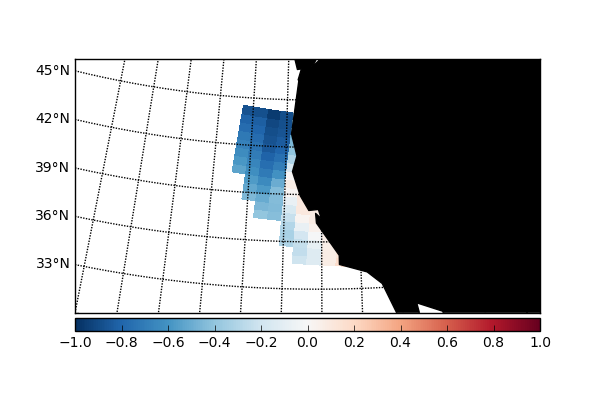
\includegraphics[width=19pc]{../../figs/CCS/study-site/calcs-study-site.png}
	\caption{Time-averaged (1920-2015) and ensemble-averaged sea-air CO$_{2}$ flux (FGCO2). Simply depicting the region over which time series are analyzed/correlated with respect to climate indices.}
\end{figure}


\bibliography{../../EBUS_BGC_Bibliography.bib}
\end{document}
